% =====================================================================
% BAB III DESKRIPSI SOLUSI
% =====================================================================

\chapter{DESKRIPSI SOLUSI}
\label{ch:deskripsi-solusi}


\section{Analisis Kebutuhan Solusi}
\label{sec:analisis-kebutuhan-solusi}

Rumusan masalah pertama menunjukkan bahwa tantangan utama AXIS bukan sekadar menjawab pesan pengguna, melainkan membangun percakapan yang terasa didengar. Mahasiswa sering menyampaikan tekanan akademik, relasi kampus, konflik keluarga, atau rasa tidak percaya diri dengan bahasa yang tidak selalu rapi. Sebagian pesan ditulis dalam bahasa Indonesia informal, sebagian mencampurkan istilah Inggris kampus, dan sebagian lagi memakai ungkapan tidak langsung ketika topiknya terasa berat. Karena itu, sistem perlu memahami cerita pengguna sebagai ekspresi personal, bukan hanya sebagai teks yang perlu dibalas.

Kebutuhan ini menuntut percakapan yang empatik, tetapi tetap berada pada batas non-klinis. AXIS perlu memvalidasi emosi, mengajak refleksi, dan menawarkan latihan ringan berdasarkan prinsip CBT tanpa menyatakan diagnosis atau mengambil peran tenaga profesional. CBT dipilih sebagai kerangka refleksi karena kajian pada Subbab~\ref{sec:cbt} menunjukkan strukturnya dapat disampaikan dalam bentuk percakapan sehari-hari tanpa kehadiran terapis, dan penyampaiannya melalui chatbot terbukti bermanfaat pada populasi mahasiswa. Pada saat yang sama, percakapan semacam ini harus tetap aman: jika pengguna menyampaikan risiko yang melewati batas pendampingan non-klinis, sistem perlu keluar dari pola dialog biasa dan mengarahkan pengguna pada bantuan yang lebih tepat.

Percakapan pendamping juga membutuhkan kendali pengguna. Jika sistem dirancang untuk digunakan berulang kali, pengguna tidak hanya berhadapan dengan respons hari ini, tetapi juga dengan jejak cerita yang mungkin dibawa ke sesi berikutnya. Karena itu, rancangan companionship tidak cukup hanya membahas empati dan memori. Sistem juga perlu memberi pilihan kepada pengguna: kapan cerita boleh menjadi memori, kapan percakapan cukup berlangsung sementara, bagaimana memori dapat dilihat atau dihapus, dan bagaimana preferensi pengalaman dapat diatur. Kendali ini penting agar personalisasi tidak berubah menjadi rasa diawasi.

Rumusan masalah kedua menambahkan dua kebutuhan yang saling melengkapi. Pengguna tidak selalu datang dengan masalah yang siap dijelaskan panjang lebar, sehingga catatan suasana hati harian membantu AXIS membaca nada awal pada hari itu. Namun mood sesaat tidak cukup untuk merefleksikan pola gejala selama dua minggu. Untuk kebutuhan yang lebih terstruktur, dipilih PHQ-9, yaitu instrumen sembilan butir yang telah tervalidasi sebagai skrining depresi \parencite{kroenke2001phq9}, termasuk pada populasi Indonesia \parencite{yulia2022phq9indo}. Penyampaiannya perlu sukarela, muncul pada waktu yang wajar, diberikan satu per satu, dan menjelaskan hasil sebagai skrining, bukan diagnosis.

Rumusan masalah ketiga menuntut memori jangka panjang. Percakapan dengan mahasiswa tidak dapat dipahami sebagai kumpulan pesan terpisah. Cerita tentang revisi skripsi hari ini bisa berkaitan dengan kegagalan presentasi bulan lalu, komentar dosen pembimbing, ekspektasi keluarga, atau perasaan tertinggal dari teman seangkatan. Jika AXIS hanya mengingat potongan teks yang mirip, hubungan semacam itu mudah hilang. Karena itu, sistem membutuhkan memori yang dapat mengenali konteks permasalahan yang relevan dalam kehidupan mahasiswa, menulis cerita pengguna, menghubungkannya dengan konteks lain, memperbaruinya ketika pemahaman pengguna berubah, dan memilih kembali memori yang relevan pada percakapan berikutnya. Pengenalan konteks tersebut berfungsi sebagai jangkar, bukan daftar topik tertutup yang dipaksakan pada setiap cerita pengguna.

Kebutuhan tersebut diringkas pada Tabel \ref{tab:kebutuhan-solusi}. Tabel ini tidak dimaksudkan menggantikan narasi, tetapi membantu menunjukkan hubungan antara masalah yang dibawa dari BAB I dan arah rancangan yang diambil pada bab ini.

\begin{table}[!htbp]
\centering
\caption{Pemetaan lima kebutuhan solusi AXIS terhadap alasan dan arah rancangan yang diambil}
\label{tab:kebutuhan-solusi}
{\footnotesize
\begin{tabularx}{\textwidth}{|>{\raggedright\arraybackslash}p{3.2cm}|>{\raggedright\arraybackslash}X|>{\raggedright\arraybackslash}X|}
\hline
\rowcolor{tableheadgray}
\textbf{Kebutuhan} & \textbf{Alasan} & \textbf{Arah rancangan} \\
\hline
K1: Respons suportif kontekstual & Pengguna membutuhkan ruang yang tidak hanya membalas pesan, tetapi memahami emosi, konteks, dan gaya bahasa. & Persona pendamping stabil, refleksi berbasis CBT non-klinis, pengayaan bahasa informal dan bahasa campur. \\
\hline
K2: Mood dan asesmen skrining depresi & Mood memberi konteks harian, sedangkan gejala dua mingguan memerlukan skrining depresi yang tervalidasi. & Mood harian sebagai konteks, PHQ-9 sebagai skrining percakapan adaptif dan sukarela. \\
\hline
K3: Memori jangka panjang & Cerita pengguna saling terkait lintas sesi dan dapat berubah makna. & Memori relasional, siklus hidup memori, dan pemilihan konteks yang relevan. \\
\hline
K4: Batas keselamatan & Chatbot pendamping tidak boleh menggantikan tenaga profesional. & Batas non-klinis, pemeriksaan risiko, dan rujukan bantuan ketika diperlukan. \\
\hline
K5: Kendali pengguna & Personalisasi dan memori jangka panjang perlu tetap terasa berada di bawah kendali pengguna. & \textit{Confession Space}, pengelolaan memori, visibilitas sensitif, preferensi respons, unduh data, dan hapus akun. \\
\hline
\end{tabularx}
}
\end{table}

Tabel \ref{tab:kebutuhan-solusi} berperan sebagai ringkasan kebutuhan pada tingkat rancangan. Rincian kebutuhan fungsional dan non-fungsional yang lebih operasional ditempatkan pada Lampiran~\ref{lamp:fr} agar BAB III tetap berfokus pada alasan dan keputusan solusi. Secara umum, AXIS juga memiliki kebutuhan non-fungsional: sistem harus dapat diaudit karena keputusan percakapan menyangkut data emosional, menjaga privasi karena pengguna menceritakan pengalaman personal, dan cukup transparan agar pengguna dapat melihat serta mengoreksi memori yang dipakai. Pada sisi pengalaman, antarmuka web dan mobile diperlukan sebagai sarana penggunaan dan pengujian, tetapi bukan pusat kontribusi penelitian. Kontribusi utama berada pada bagaimana percakapan, mood, PHQ-9, dan memori jangka panjang diorkestrasikan menjadi satu sistem pendamping.

K1, K2, dan K3 merupakan turunan langsung dari tiga rumusan masalah pada BAB I. K4 dan K5 tidak menambah rumusan masalah baru, melainkan menjadi kebutuhan lintas-rumusan: batas keselamatan menjaga seluruh bentuk percakapan tetap non-klinis, sedangkan kendali pengguna menjaga personalisasi dan memori tetap berada di bawah keputusan pengguna.

\section{Gambaran Umum Solusi}
\label{sec:gambaran-umum}

AXIS dirancang sebagai chatbot pendamping non-klinis untuk mahasiswa Indonesia, dengan pengguna mahasiswa sebagai aktor utamanya. Dari sudut pandang pengguna, terdapat delapan kelompok interaksi: bercerita dan berefleksi dalam percakapan, berbicara di ruang suara sementara, mencatat suasana hati harian, mengisi skrining PHQ-9, melakukan latihan reflektif, melihat dan mengelola memori, mengakses bantuan dan hotline, serta mengatur akun dan data pribadi. Diagram \textit{use case} pada Gambar \ref{fig:solution-use-case} merangkum kedelapan interaksi tersebut.

\begin{figure}[!htbp]
  \centering
  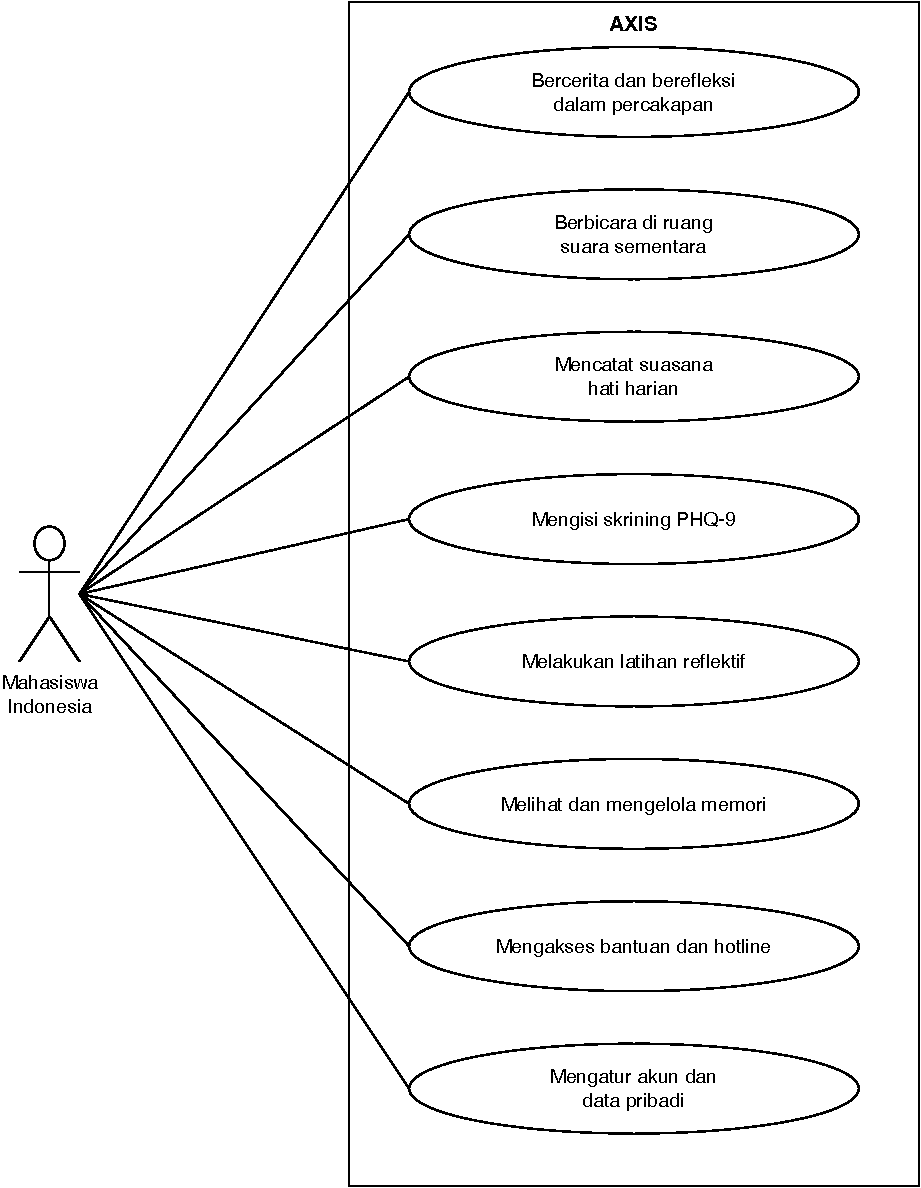
\includegraphics[width=0.8\textwidth,height=0.72\textheight,keepaspectratio]{figures/solution_use_case.pdf}
  \caption[Diagram use case AXIS]{Diagram \textit{use case} AXIS sebagai chatbot pendamping non-klinis untuk mahasiswa Indonesia.}
  \label{fig:solution-use-case}
\end{figure}

Alur penggunaan kedelapan interaksi tersebut ditunjukkan pada Gambar \ref{fig:solution-overview-flow}. Pengguna memilih ruang sesuai kebutuhannya saat itu, setiap giliran percakapan melewati pemeriksaan keselamatan, dan respons selalu berada pada batas non-klinis. Ketika sesi berakhir, hanya sesi yang layak yang ditulis menjadi memori jangka panjang. Percakapan di ruang suara sementara mengikuti alur yang sama, tetapi tidak pernah meninggalkan memori.

\begin{figure}[!htbp]
  \centering
  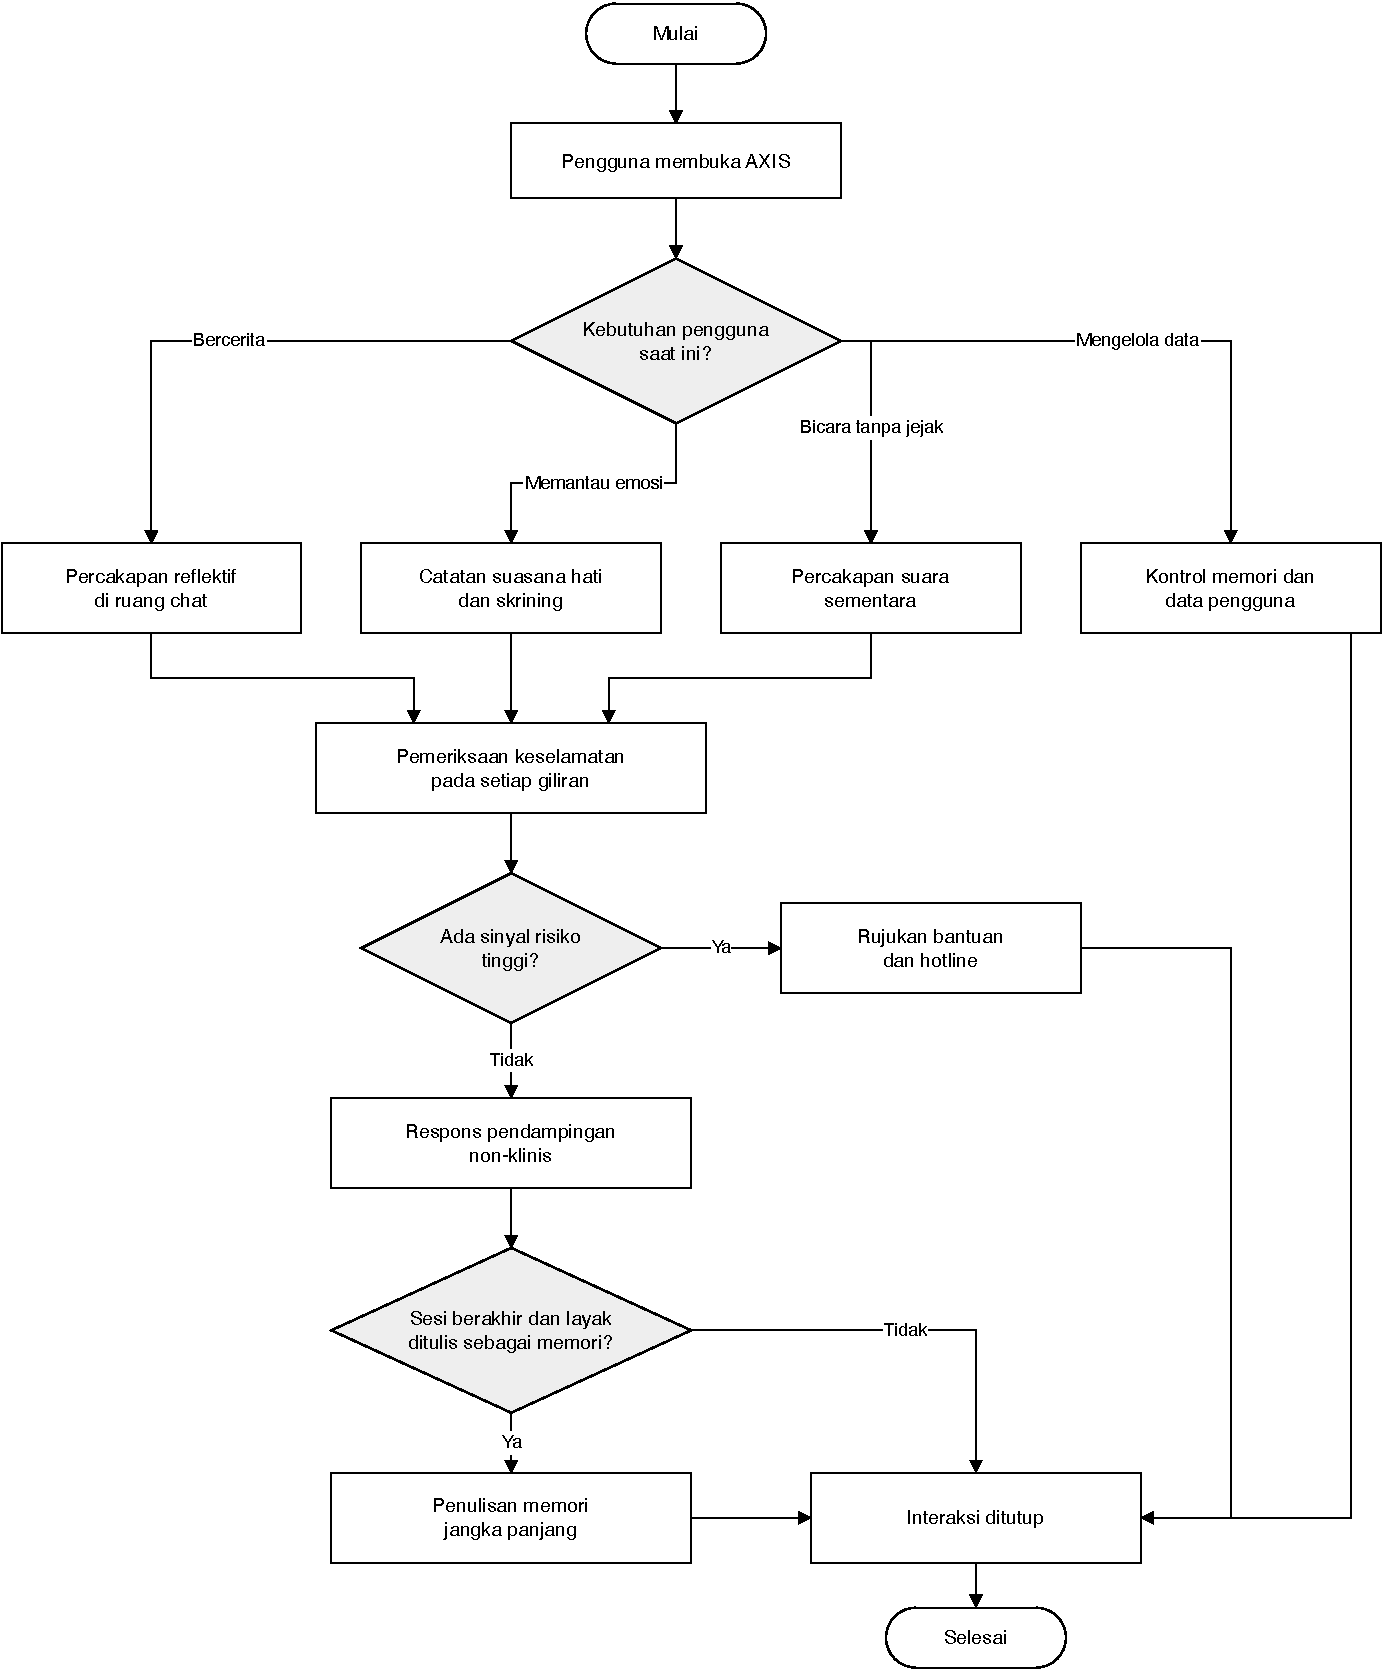
\includegraphics[width=0.92\textwidth]{figures/solution_overview_flow.pdf}
  \caption[Flowchart penggunaan AXIS]{\textit{Flowchart} konseptual penggunaan AXIS dari pembukaan aplikasi hingga penulisan memori jangka panjang.}
  \label{fig:solution-overview-flow}
\end{figure}

Rancangan AXIS tidak memandang fitur-fitur tersebut sebagai daftar kemampuan yang berdiri sendiri, melainkan sebagai satu kesatuan peran \textit{companionship} yang saling melengkapi, dari ruang bercerita utama hingga kendali pengguna atas data personalnya. Tabel \ref{tab:peran-fitur-companionship} memetakan peran masing-masing fitur tersebut.

\begin{table}[!htbp]
\centering
\caption{Peran fitur dalam pengalaman companionship AXIS}
\label{tab:peran-fitur-companionship}
{\footnotesize
\begin{tabularx}{\textwidth}{|>{\raggedright\arraybackslash}p{3.2cm}|>{\raggedright\arraybackslash}X|}
\hline
\rowcolor{tableheadgray}
\textbf{Fitur} & \textbf{Peran dalam companionship} \\
\hline
Chat utama & Ruang bercerita dan refleksi yang mempertahankan konteks lintas sesi. \\
\hline
\textit{Confession Space} & Percakapan suara sementara yang isinya tidak dimasukkan ke memori jangka panjang AXIS. \\
\hline
Mood harian & Sinyal ringan mengenai suasana hati pengguna pada hari tertentu. \\
\hline
PHQ-9 & Skrining terstruktur yang membantu pengguna melihat kondisi dua minggu terakhir tanpa klaim diagnosis. \\
\hline
Memori dan peta memori & Transparansi terhadap apa yang diingat sistem serta kesempatan untuk mengoreksi atau menghapusnya. \\
\hline
Profil dan preferensi & Penyesuaian nama panggilan, bahasa percakapan, suara, dan mode respons agar AXIS terasa lebih sesuai dengan pengguna. \\
\hline
Bantuan, hotline, dan pengaturan & Penjelasan batas sistem, rujukan bantuan, reset memori, unduh data, hapus riwayat, dan hapus akun. \\
\hline
\end{tabularx}
}
\end{table}

Tabel tersebut juga menetapkan posisi fitur kontrol pengguna, yang menjawab K5 pada Tabel~\ref{tab:kebutuhan-solusi}. Fitur seperti hapus memori, unduh data, hapus akun, visibilitas sensitif, dan preferensi respons bukan kontribusi algoritmik yang berdiri sendiri. Perannya menjaga agar personalisasi tidak berubah menjadi pengalaman yang terasa mengawasi. Kendali pengguna dengan demikian menjadi syarat sosial dari \textit{companionship}: sistem boleh mengingat pengguna sejauh pengguna tetap dapat melihat, mengatur, dan menghentikan ingatan tersebut.

\subsection{Rancangan Peran \textit{Companionship Chatbot}}
\label{sec:rancangan-companionship}

Rancangan berikut menjawab K1 pada Tabel~\ref{tab:kebutuhan-solusi}. Peran AXIS sebagai \textit{companionship chatbot} dibangun dari prinsip bahwa pengguna tidak selalu membutuhkan solusi langsung. Sering kali pengguna membutuhkan ruang untuk menyusun ulang cerita, merasa didengar, dan memahami perasaan yang sedang muncul. Karena itu, respons AXIS dirancang untuk mendahulukan validasi emosi, pertanyaan terbuka, dan tawaran refleksi yang tidak memaksa.

Prinsip CBT dipakai sebagai kerangka refleksi, bukan sebagai terapi. AXIS dapat membantu pengguna melihat hubungan antara situasi, pikiran, emosi, dan perilaku. Jika pengguna menunjukkan kritik diri, sistem dapat mengajak pengguna melihat cara bicara kepada diri sendiri. Jika pengguna menunjukkan kepanikan, sistem dapat menawarkan latihan penjangkaran (\textit{grounding}). Jika pengguna menunjukkan pikiran katastrofik, sistem dapat mengajak pengguna menimbang kemungkinan lain. Semua latihan tersebut tetap berada dalam batas non-klinis dan harus terasa sebagai undangan, bukan kewajiban.

Perancangan respons reflektif ini memisahkan proses secara eksplisit menjadi dua tahap berurutan: memahami, baru kemudian menyuarakan. Pemisahan ini mengikuti pembedaan empati kognitif dan empati belas kasih pada Subbab~\ref{subsec:model-empati} \parencite{decetyCowell2014}, karena memahami mengapa pengguna merasakan sesuatu dalam konteks yang spesifik adalah proses yang berbeda dari memutuskan tindakan respons yang membantu. Tahap pemahaman menyusun model psikologis pengguna dari memori yang tersedia mengikuti struktur situasi-emosi-pikiran-perilaku pada model \textit{hot cross bun} \parencite{greenbergerPadesky1995}, memperlakukan distorsi kognitif yang terdeteksi sebagai skema yang dapat dievaluasi terprogram \parencite{beck1979}, tanpa pernah menyusun kalimat balasan itu sendiri. Tahap penyuaraan menerima hasil pemahaman tersebut dan menerjemahkannya menjadi kalimat yang hangat, tanpa pernah menyebutkan mekanisme analisis yang mendasarinya kepada pengguna. Pemisahan ini dirancang agar kedalaman pemahaman memperkaya ketepatan dan nada respons, bukan ditunjukkan sebagai proses analitis yang terlihat pengguna.

Alur pemilihan teknik ditunjukkan pada Gambar \ref{fig:cbt-dialogue-flow}. Teknik tidak dipilih sebagai langkah otomatis yang selalu muncul. Sistem lebih dahulu memeriksa apakah percakapan sedang berada dalam alur skrining atau kondisi risiko, menghormati penolakan yang baru saja diberikan pengguna, menimbang apakah muatan emosi dan kesiapan pengguna sudah cukup, dan baru memilih teknik yang sesuai dengan sinyal dominan pada pesan. Dengan cara ini, CBT memperkaya percakapan tanpa memaksa pengguna masuk ke format latihan.

\begin{figure}[!htbp]
  \centering
  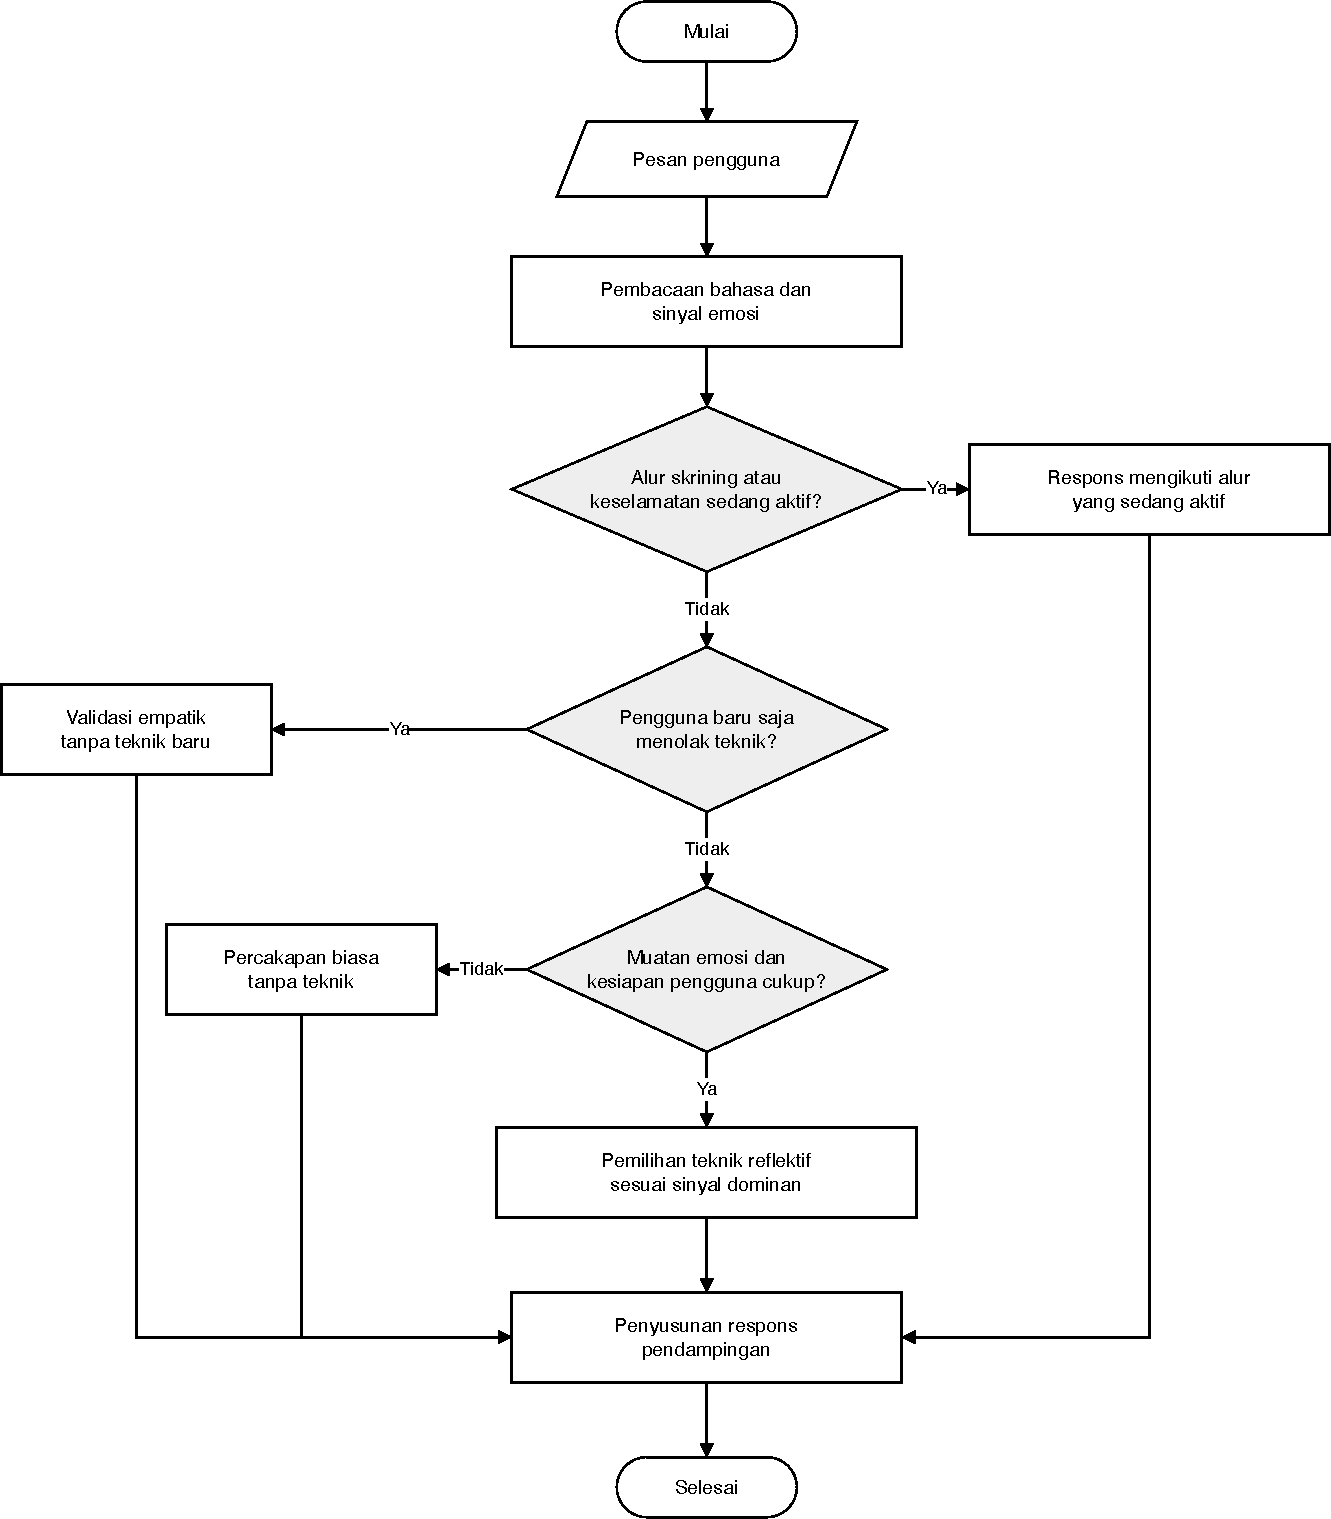
\includegraphics[width=0.85\textwidth]{figures/cbt_dialogue_flow.pdf}
  \caption[Flowchart pemilihan teknik reflektif]{\textit{Flowchart} konseptual pemilihan teknik reflektif non-klinis dalam percakapan AXIS.}
  \label{fig:cbt-dialogue-flow}
\end{figure}

Bentuk teknik yang tersedia beserta sinyal percakapan yang memicunya dirangkum pada Tabel \ref{tab:pemetaan-teknik-reflektif}. Ketujuh bentuk ini diturunkan dari teknik CBT yang diulas pada Subbab~\ref{sec:cbt}, disesuaikan menjadi tawaran percakapan singkat yang dapat diterima atau ditolak pengguna.

\begin{table}[!htbp]
\centering
\caption{Pemetaan sinyal percakapan ke teknik reflektif}
\label{tab:pemetaan-teknik-reflektif}
{\footnotesize
\begin{tabularx}{\textwidth}{|>{\raggedright\arraybackslash}p{5.6cm}|>{\raggedright\arraybackslash}X|}
\hline
\rowcolor{tableheadgray}
\textbf{Sinyal dominan pada pesan} & \textbf{Bentuk respons reflektif} \\
\hline
Emosi umum tanpa pola pikir tertentu & Validasi empatik dan pertanyaan terbuka. \\
\hline
Pola pikir menyimpang, misalnya katastrofik & Ajakan menimbang kemungkinan lain (\textit{reframing}). \\
\hline
Pikiran otomatis yang terus berulang & Catatan pikiran bertahap (\textit{thought record}). \\
\hline
Kritik diri yang berulang & Latihan berbicara lebih lembut kepada diri sendiri (\textit{self-compassion}). \\
\hline
Distres akut atau kepanikan & Latihan penjangkaran singkat (\textit{grounding}). \\
\hline
Kecenderungan menghindar atau menarik diri & Ajakan mengambil satu langkah kecil yang terjangkau (\textit{behavior activation}). \\
\hline
Permintaan penjelasan konsep emosional & Penjelasan singkat tanpa label klinis (\textit{psychoeducation}). \\
\hline
\end{tabularx}
}
\end{table}

Tabel \ref{tab:pemetaan-teknik-reflektif} menyajikan tiap sinyal sebagai baris independen, tetapi pada percakapan nyata lebih dari satu sinyal dapat muncul bersamaan pada satu pesan yang sama, misalnya pikiran katastrofik yang diutarakan bersamaan dengan afek akut (jantung berdebar, panik). Untuk kondisi ini, rancangan AXIS memprioritaskan regulasi afek akut (\textit{grounding}) di atas penantangan pola pikir (\textit{reframing}), mengikuti prinsip dialectical behavior therapy bahwa penalaran yang ditawarkan saat afek sedang sangat aktif cenderung kurang efektif diterima \parencite{linehan1993dbt}. Prioritas ini konsisten, tetapi berarti distorsi kognitif yang muncul bersamaan afek akut tidak langsung ditantang pada giliran yang sama. Agar distorsi tersebut tidak hilang begitu saja setelah giliran \textit{grounding}, sistem menyimpan nama distorsi yang terdeteksi bersamaan sinyal akut tadi, lalu secara otomatis menawarkan \textit{reframing} pada giliran berikutnya jika pengguna masih menunjukkan muatan emosional dan belum berpindah topik. Mekanisme susulan ini diverifikasi berjalan pada pemanggilan LLM nyata (Subbab~\ref{subsec:impl-pipeline-agentik}).

Ruang percakapan suara sementara yang diperkenalkan pada BAB I disebut \textit{Confession Space} pada rancangan AXIS. Fitur ini dirancang untuk situasi ketika pengguna lebih nyaman berbicara daripada mengetik. Rancangan ini berangkat dari landasan pada Subbab~\ref{subsec:landasan-confession-space}: nilai bercerita tidak selalu bergantung pada apakah cerita tersebut diingat, sehingga kanal yang sengaja tidak menulis isi percakapan ke memori jangka panjang tetap memberi manfaat tersendiri. Fitur ini berupa percakapan suara dengan hasil transkripsi yang ditampilkan sebagai takarir agar pengguna dapat mengikuti isi percakapan secara visual.

Perbedaan utamanya dari chat biasa terletak pada batas persistensi. Isi pesan dan transkrip hanya dipakai sebagai konteks selama percakapan berlangsung, tidak dijadikan riwayat permanen maupun memori personal AXIS. Batas ini disampaikan secara jujur: audio tetap diproses oleh layanan transkripsi dan sintesis suara pihak ketiga, dan metadata operasional minimum seperti keberadaan sesi serta penanda keselamatan tetap dicatat. Pengguna memperoleh ruang yang lebih ringan tanpa diberi janji privasi yang melampaui kendali AXIS, dan batas keselamatan tetap berlaku penuh: jika terdapat risiko tinggi, sistem tetap mengarahkan pengguna ke bantuan yang sesuai.
\label{subsec:rancangan-confession-space}

Kendali pengguna menjadi bagian dari rancangan companionship karena AXIS membawa memori personal ke dalam percakapan. Pengguna perlu dapat melihat memori yang tersimpan, menyembunyikan informasi sensitif dari tampilan, memperbarui atau menghapus catatan yang tidak lagi tepat, serta menghapus riwayat atau akun ketika tidak ingin melanjutkan penggunaan. Pilihan-pilihan ini bukan pusat kontribusi algoritmik, tetapi menjadi syarat agar kontribusi memori jangka panjang dapat diterima dalam pengalaman pendampingan.

\subsection{Rancangan Percakapan Reflektif dan Persona}
\label{sec:rancangan-percakapan-persona}
\label{sec:rancangan-axis}

Rancangan berikut memperdalam K1 pada Tabel~\ref{tab:kebutuhan-solusi} dari sisi stabilitas persona dan kalibrasi domain. Persona AXIS dirancang stabil lintas sesi. Stabilitas ini penting karena pengguna yang kembali setelah beberapa hari atau minggu perlu merasa berhadapan dengan pendamping yang sama, bukan agen yang berubah-ubah. AXIS harus terdengar hangat, tidak menghakimi, tidak terlalu formal, tetapi juga tidak berpura-pura menjadi manusia atau tenaga klinis. Dalam konteks mahasiswa Indonesia, respons perlu cukup natural untuk menerima bahasa informal dan bahasa campur, tetapi tetap jelas ketika membahas topik yang sensitif.

Kalibrasi mahasiswa Indonesia tidak berarti sistem hanya bisa digunakan mahasiswa. Artinya, rancangan awal dipusatkan pada domain yang secara empiris paling banyak muncul pada kehidupan mahasiswa: tekanan akademik dan relasi dengan dosen pembimbing \parencite{pusparini2025thesisstress}, tekanan dan ekspektasi keluarga \parencite{mardhiyah2026parentalpressure}, keterlibatan organisasi yang berisiko \textit{burnout} \parencite{octaviani2023organizationalburnout,haase2025feelingseen}, pembentukan identitas diri dan rasa tertinggal dari teman seangkatan \parencite{pakozdy2024impostor,habibie2023quarterlifecrisis}, serta ketidakpastian transisi karier \parencite{yang2025employmentanxiety}. Domain ini diturunkan dari literatur tersebut, lalu dipakai secara konsisten untuk memengaruhi kategori memori yang dirancang pada Subbab~\ref{sec:rancangan-memori-jangka-panjang}, contoh label topik pada instruksi ekstraksi memori (Lampiran~\ref{lamp:agentic-prompts-kg}), gaya bahasa, dan sumber bantuan yang disediakan.

Kalibrasi ini tidak berhenti pada label topik. Kategori Subjek membedakan dosen pembimbing skripsi dari dosen wali karena keduanya berperan berbeda dalam pengalaman mahasiswa \parencite{sherlywati2022academicadvisor}, serta mengenali pengelola dan teman kos sebagai sumber dukungan atau tekanan sosial bagi mahasiswa perantauan \parencite{putri2025boardinghouse}. Kategori pemicu diperluas mencakup tekanan tempat tinggal di samping akademik, keluarga, organisasi, karier, dan finansial. Kategori perilaku mengacu pada pola \textit{coping} yang terdokumentasi pada mahasiswa Indonesia, seperti prokrastinasi akademik dan penghindaran terhadap dosen pembimbing \parencite{fernanda2025procrastination}. Dengan demikian, kalibrasi domain diterapkan konsisten pada seluruh kategori memori pada Tabel \ref{tab:kategori-memori}, bukan hanya pada satu kategori.

Tidak seluruh kategori memerlukan kosakata tetap, dan ketiadaan itu adalah keputusan rancangan, bukan celah yang terlewat. Catatan Pengalaman, Pikiran, dan Emosi tetap ditulis mendekati kata-kata asli pengguna karena tujuannya merekam narasi personal apa adanya. Ketiganya hanya diberi contoh pengenalan pola kehidupan mahasiswa yang umum terjadi, seperti sidang yang ditolak, rasa tidak pantas melanjutkan studi, atau rasa bersalah terkait beban finansial keluarga, agar pola yang memang muncul tidak luput dicatat tanpa memaksakan frasa baku menggantikan kata-kata pengguna. Hasil PHQ-9 sengaja tidak dikalibrasi sama sekali karena instrumen skrining harus konsisten lintas populasi agar tetap valid. Ringkasan sesi justru diperkuat instruksinya agar mempertahankan detail relasi yang spesifik, misalnya tetap membedakan dosen pembimbing dari dosen wali alih-alih meratakan keduanya menjadi ``masalah akademik''. Kalibrasi ini ditutup pada sisi penyusunan respons: peran yang berbeda pada memori tetap dihormati perbedaannya saat direfleksikan kembali ke pengguna.

\subsection{Rancangan Mood Harian dan Asesmen Skrining Depresi PHQ-9}
\label{subsec:rancangan-mood-phq9}
\label{subsec:rancangan-jitai-gate}
\label{subsec:rancangan-state-phq9}
\label{subsec:rancangan-eskalasi-item9}

Rancangan berikut menjawab K2 pada Tabel~\ref{tab:kebutuhan-solusi}. Sinyal ringan dari percakapan sehari-hari cukup untuk menangkap nada emosional pengguna saat itu, tetapi tidak cukup untuk menilai kondisi yang berkembang selama beberapa minggu. Menilai perkembangan semacam ini dengan pertanyaan buatan sendiri berisiko menghasilkan skrining yang hasilnya sulit dipertanggungjawabkan, karena tidak ada dasar empiris atas ambang maupun tafsir skornya. Kebutuhan inilah yang mengarahkan rancangan pada instrumen skrining tervalidasi. Di antara instrumen skrining depresi yang tersedia, PHQ-9 dipilih karena bentuknya ringkas (sembilan butir), telah tervalidasi luas termasuk pada populasi mahasiswa Indonesia, dan pada sistem sejenis terbukti dapat disampaikan lewat percakapan tanpa kehilangan konsistensi hasil pengukurannya (Subbab~\ref{subsec:phq9-instrumen}).

Mood harian dirancang sebagai pemeriksaan ringan yang melengkapi PHQ-9 pada level harian. Pengguna dapat memilih satu dari lima kondisi, dari sangat sedih hingga sangat senang. Nilai ini tidak diperlakukan sebagai asesmen klinis, melainkan sebagai konteks awal yang membantu AXIS menyesuaikan nada percakapan. Jika pengguna beberapa hari berturut-turut memilih mood rendah, sistem dapat lebih berhati-hati dalam merespons dan menunda respons yang terlalu optimistis.

PHQ-9 sendiri ditempatkan pada level yang lebih terstruktur, dengan penawaran yang diatur mengikuti prinsip JITAI (Subbab~\ref{subsec:jitai}) agar tidak muncul pada waktu yang salah. Prinsip tersebut diterjemahkan menjadi tiga gerbang penawaran yang dirangkum pada Tabel \ref{tab:gerbang-phq9}. Di luar ketiganya, tawaran juga muncul ketika pengguna memintanya secara langsung. Alur mood harian dan PHQ-9 secara keseluruhan ditunjukkan pada Gambar \ref{fig:phq9-state-machine}.

\begin{table}[!htbp]
\centering
\caption{Tiga gerbang penawaran skrining PHQ-9}
\label{tab:gerbang-phq9}
{\footnotesize
\begin{tabularx}{\textwidth}{|>{\raggedright\arraybackslash}p{2.6cm}|>{\raggedright\arraybackslash}X|>{\raggedright\arraybackslash}X|}
\hline
\rowcolor{tableheadgray}
\textbf{Gerbang} & \textbf{Aturan} & \textbf{Alasan rancangan} \\
\hline
Pemanasan dialog & Tawaran pertama baru muncul setelah beberapa giliran percakapan awal, bukan pada pesan pertama. & Skrining yang datang sebelum percakapan terbangun terasa seperti formulir, bukan pendampingan. \\
\hline
Jadwal berkala & Siklus rutin setiap 14 hari. & PHQ-9 menanyakan kondisi dua minggu terakhir, sehingga siklus penawaran mengikuti jendela pengukuran instrumen. \\
\hline
Jeda adaptif & Setelah penolakan, tawaran ulang ditunda. Jeda memendek ketika distres akut terdeteksi dan memanjang ketika pola memburuk terlihat dari riwayat. & Tawaran yang diulang terlalu cepat terasa memaksa dan melanggar prinsip kesukarelaan skrining. \\
\hline
\end{tabularx}
}
\end{table}

\begin{figure}[!htbp]
  \centering
  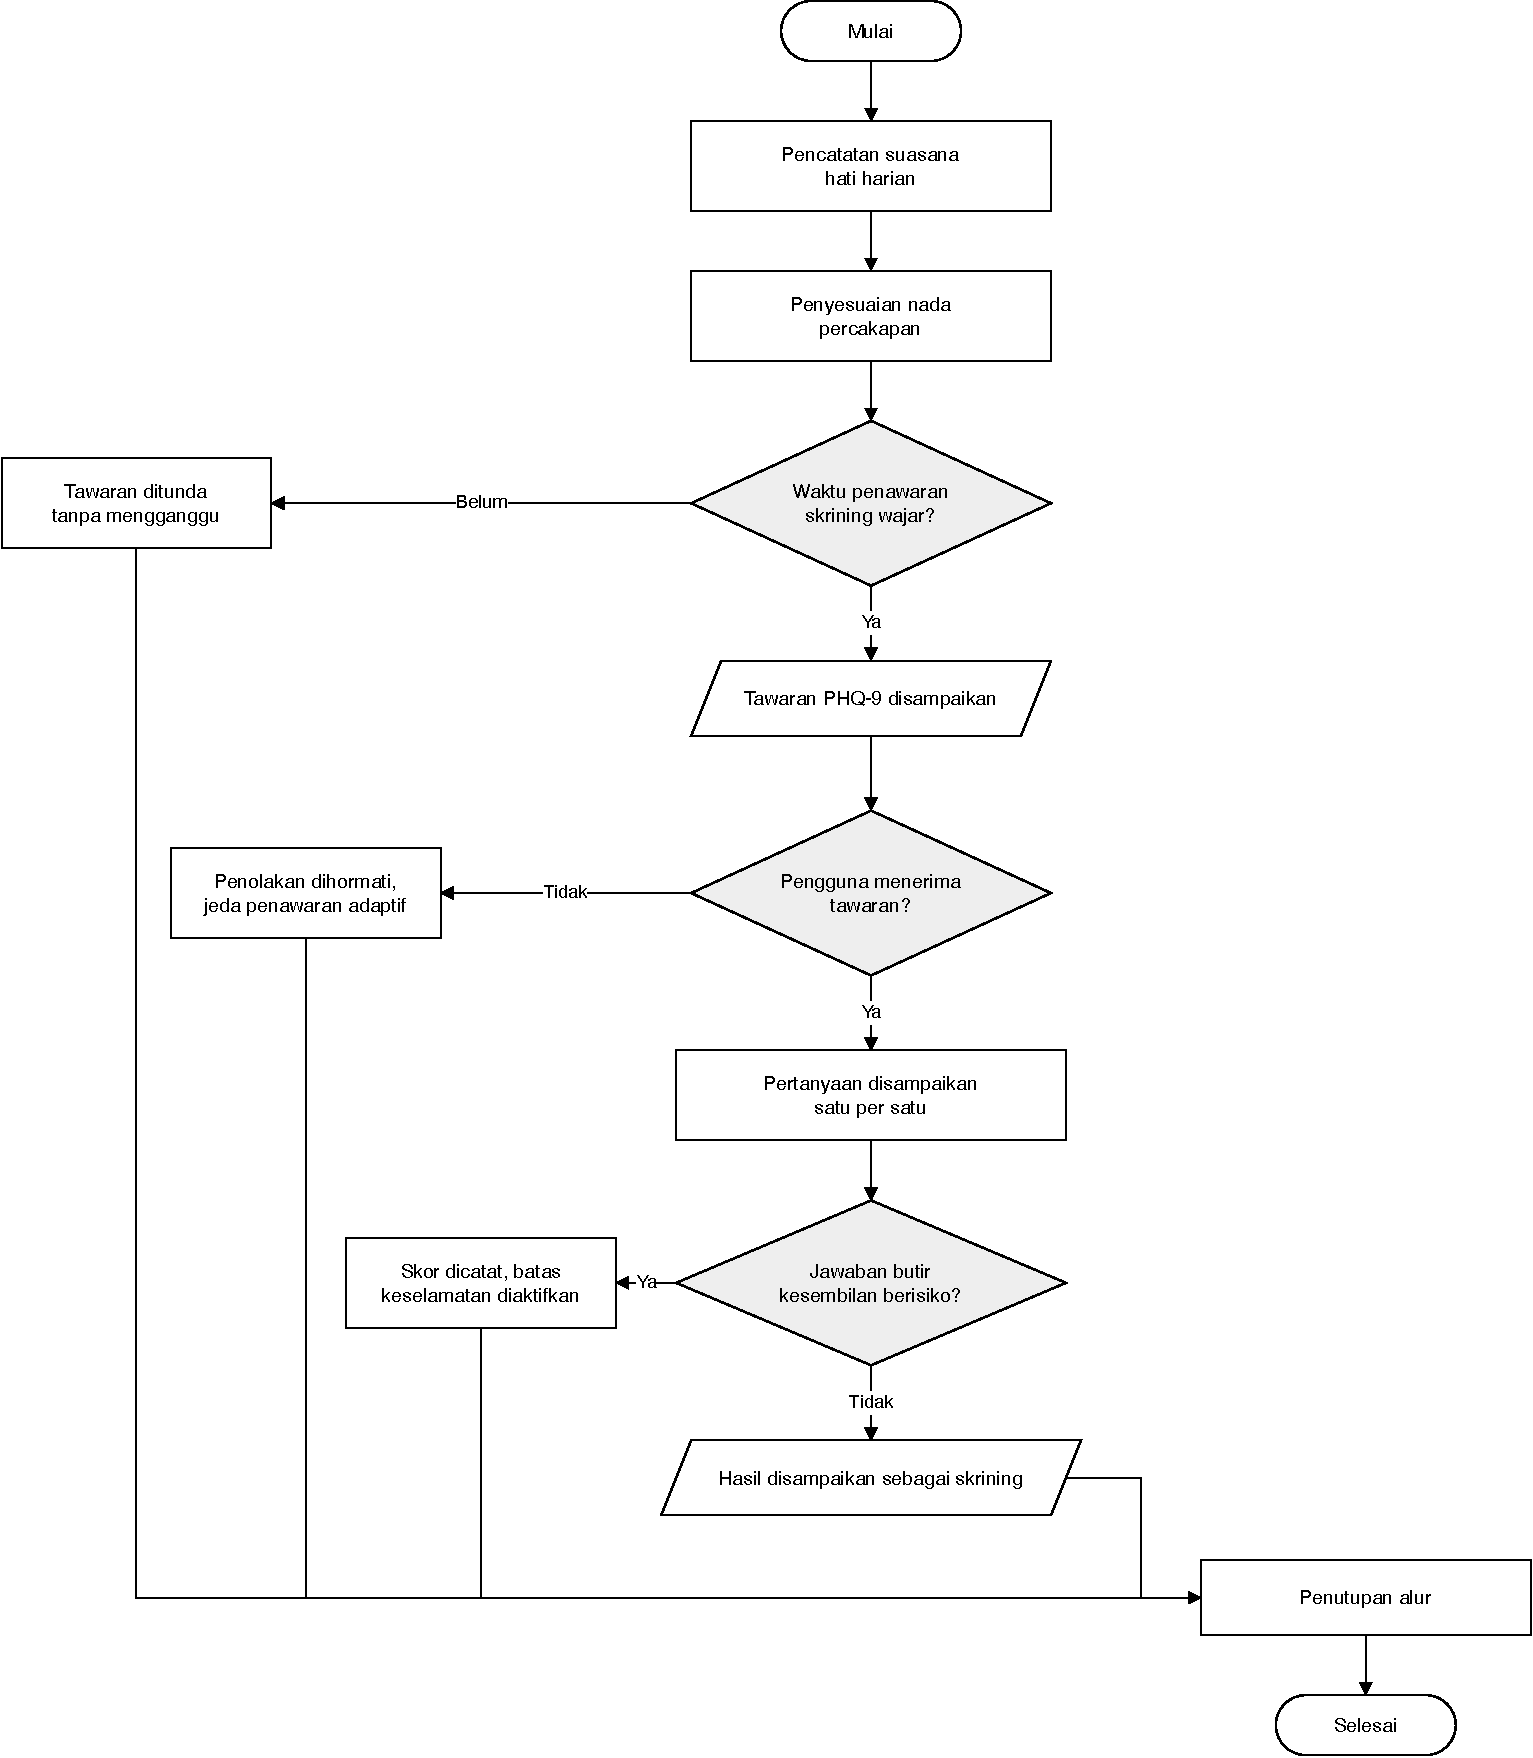
\includegraphics[width=0.85\textwidth]{figures/phq9_concept_flow.pdf}
  \caption[Flowchart mood harian dan asesmen PHQ-9]{\textit{Flowchart} konseptual mood harian dan asesmen skrining depresi PHQ-9 secara percakapan bertahap.}
  \label{fig:phq9-state-machine}
\end{figure}

Hasil PHQ-9 harus disampaikan dengan bahasa skrining. AXIS tidak menyatakan bahwa pengguna mengalami depresi atau gangguan tertentu. Sistem hanya menyampaikan bahwa skor dapat menjadi sinyal untuk memperhatikan kondisi diri, menjaga dukungan sosial, dan mencari bantuan profesional bila diperlukan. Apabila jawaban pada butir kesembilan menunjukkan risiko, sistem menyelesaikan perhitungan dan pencatatan hasil skrining pada giliran yang sama, kemudian langsung mengalihkan alur ke batas keselamatan sebelum percakapan normal dapat dilanjutkan. Dengan demikian, eskalasi tidak memotong administrasi instrumen di tengah jalan, tetapi juga tidak ditunda ke interaksi pengguna berikutnya.

\subsection{Rancangan Memori Jangka Panjang dan \textit{Lifecycle}}
\label{sec:rancangan-memori-jangka-panjang}
\label{sec:rancangan-siklus-memori}

Rancangan berikut menjawab K3 pada Tabel~\ref{tab:kebutuhan-solusi}. Memori AXIS dirancang untuk menjawab pertanyaan yang tidak dapat diselesaikan oleh riwayat chat biasa: apa yang pernah dialami pengguna, siapa yang terlibat, emosi apa yang muncul, pikiran apa yang sering berulang, dan bagaimana makna suatu pengalaman berubah dari waktu ke waktu. Karena itu, memori dibentuk sebagai arsitektur hibrid berbasis \textit{knowledge graph}: relasi antarmemori menjadi sumber utama pemahaman konteks, sedangkan pencarian semantik membantu menemukan kandidat memori yang relevan. Pilihan ini mengikuti dua temuan kajian pustaka. Pencarian kemiripan semantik saja kesulitan menjawab pertanyaan relasional dan temporal (Subbab~\ref{subsec:rag-keterbatasan}), sementara penggabungan graf dengan pencarian semantik menutupi kelemahan masing-masing pendekatan (Subbab~\ref{subsec:hybrid-retrieval}). Alur penulisan dan siklus hidup memori ditunjukkan pada Gambar \ref{fig:memory-concept-flow}.

\begin{figure}[!htbp]
  \centering
  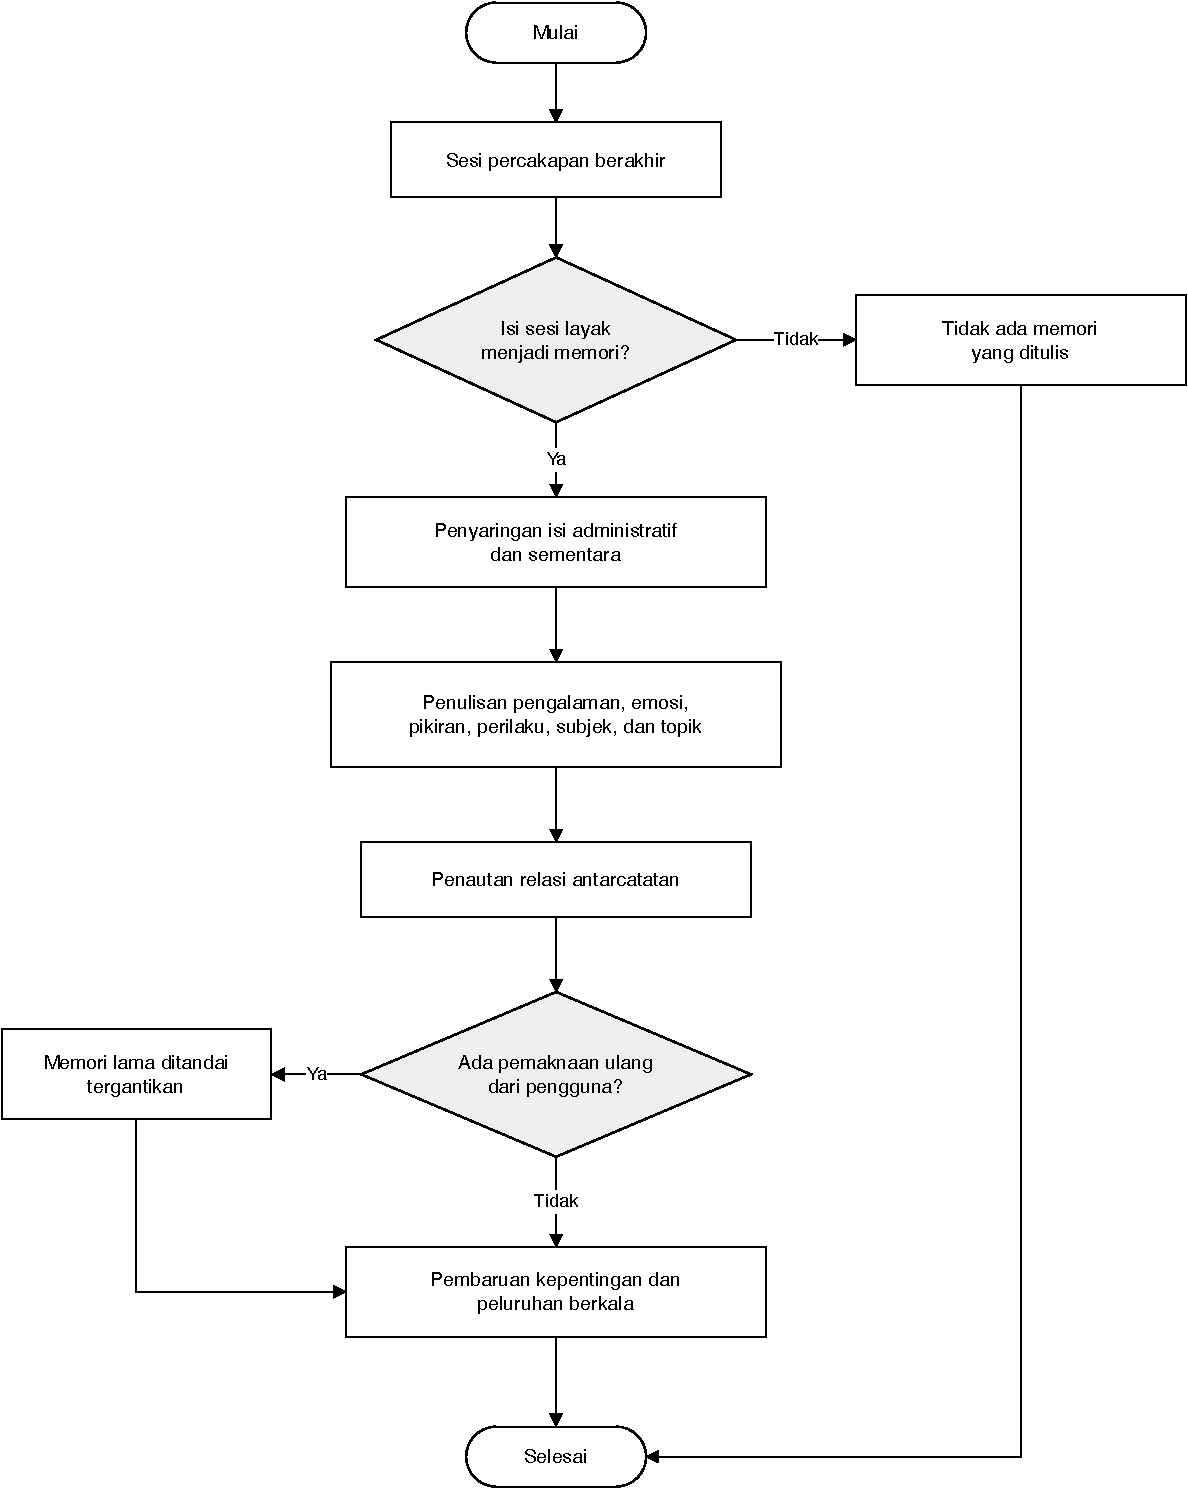
\includegraphics[width=0.85\textwidth]{figures/memory_concept_flow.pdf}
  \caption[Flowchart penulisan dan siklus hidup memori]{\textit{Flowchart} konseptual penulisan dan siklus hidup memori jangka panjang AXIS.}
  \label{fig:memory-concept-flow}
\end{figure}

Penggunaan graf pada rancangan ini tidak dibatasi hanya sebagai pengaya representasi setelah kandidat memori ditemukan. Mengikuti prinsip \textit{spreading activation} \parencite{collinsloftus1975} pada Subbab~\ref{subsec:hybrid-retrieval}, penelusuran graf juga dirancang untuk berperan pada tahap penemuan kandidat itu sendiri: dari satu memori benih yang ditemukan pencarian semantik, penelusuran satu langkah ke entitas relasi yang sama (Pemicu atau Subjek yang identik) dapat menemukan pengalaman lain milik pengguna yang sama sekali tidak mirip secara leksikal maupun semantik dengan pesan pengguna saat itu, tetapi terhubung secara nyata lewat identitas relasi yang sama pada graf. Kemampuan ini dirancang khusus untuk jenis kueri yang secara struktural tidak dapat dijawab pencarian semantik semata, terlepas dari besar korpus atau kualitas model \textit{embedding} yang dipakai.

Keputusan memakai memori relasional membawa konsekuensi. Sistem perlu menjaga struktur, sinkronisasi, dan relevansi memori. Namun, konsekuensi tersebut diterima karena memori personal tidak berbentuk daftar fakta yang statis. Mahasiswa dapat mengubah cara memaknai pengalaman. Dosen yang awalnya terasa menekan bisa kemudian dipahami sebagai pembimbing yang peduli, dan revisi yang awalnya terasa gagal bisa kemudian dipahami sebagai proses memperbaiki karya. Jika memori tidak memiliki \textit{lifecycle}, sistem berisiko mengulang pemahaman lama yang tidak lagi tepat.

\textit{Lifecycle} memori pada tingkat rancangan memiliki tiga tujuan. Pertama, memori baru hanya ditulis ketika percakapan sudah cukup jelas dan tidak bersifat sementara. Kedua, memori lama dapat ditutup ketika pengguna memberi \textit{reframe}, koreksi, atau resolusi baru. Ketiga, memori yang lama tidak digunakan perlu turun kepentingannya agar tidak terus mendominasi percakapan. Rancangan ini menjaga agar memori jangka panjang tidak sekadar bertambah, tetapi juga dapat matang mengikuti perubahan cerita pengguna.

Secara operasional, memori jangka panjang pada penelitian ini didefinisikan sebagai kemampuan arsitektur mempertahankan dan memanfaatkan konteks pengguna melampaui batas satu sesi percakapan, dengan jendela dukungan dari 14 hari hingga enam bulan. Batas bawah 14 hari mengikuti satu siklus penuh skrining PHQ-9 yang dirancang pada Subbab~\ref{subsec:rancangan-mood-phq9}, dan selaras dengan temuan \textcite{bickmorePicard2005} bahwa kepercayaan antara pengguna dan agen percakapan baru terbentuk setelah beberapa sesi berulang dalam rentang berminggu-minggu. Batas atas enam bulan mengikuti jendela peluruhan dan pengarsipan memori yang ditetapkan pada kebutuhan fungsional sistem (Lampiran~\ref{lamp:fr}).

Kategori memori yang dipakai AXIS dirancang untuk menonjolkan konteks mahasiswa Indonesia. Tabel \ref{tab:kategori-memori} menunjukkan peran setiap kategori pada tingkat rancangan.

\begin{table}[!htbp]
\centering
\caption{Kategori memori dan perannya dalam konteks mahasiswa Indonesia}
\label{tab:kategori-memori}
{\footnotesize
\begin{tabularx}{\textwidth}{|>{\raggedright\arraybackslash}p{2.7cm}|>{\raggedright\arraybackslash}X|>{\raggedright\arraybackslash}X|}
\hline
\rowcolor{tableheadgray}
\textbf{Kategori} & \textbf{Yang dicatat} & \textbf{Contoh konteks mahasiswa} \\
\hline
Pengalaman & Peristiwa yang diceritakan pengguna. & Sidang, revisi, organisasi, konflik teman, tekanan keluarga. \\
\hline
Emosi & Perasaan dan intensitas yang menyertai pengalaman. & Cemas sebelum ujian, malu setelah presentasi, lega setelah konsultasi. \\
\hline
Pikiran & Tafsir atau pikiran otomatis pengguna. & ``Aku pasti gagal'', ``Aku tertinggal dari teman'', ``Aku tidak cocok di jurusan ini''. \\
\hline
Rekam pikiran & Catatan reflektif 5-langkah CBT beserta wawasan (\textit{insight}) yang diperoleh pengguna. & Situasi revisi ditolak, pikiran otomatis ``aku gagal total'', bukti pendukung/penyangkal, wawasan bahwa satu penolakan bukan kegagalan total. \\
\hline
Perilaku & Respons atau kebiasaan yang muncul, termasuk pola \textit{coping} yang didokumentasikan pada mahasiswa Indonesia \parencite{fernanda2025procrastination}. & Menunda revisi skripsi, begadang, menghindari dosen pembimbing, menarik diri ke kamar kos, mencari teman cerita. \\
\hline
Subjek & Orang, tempat, hewan, benda, atau entitas penting, termasuk peran spesifik lingkungan kampus dan tempat tinggal mahasiswa perantauan \parencite{sherlywati2022academicadvisor,putri2025boardinghouse}. & Dosen pembimbing skripsi, dosen wali (peran berbeda dari dosen pembimbing), teman sekelompok, senior organisasi, ibu/bapak kos, teman satu kos, keluarga. \\
\hline
Topik & Tema berulang yang menyatukan memori. & Tekanan akademik, harga diri, isolasi sosial, relasi kampus, tekanan tempat tinggal/rantau. \\
\hline
Memori ringkas & Kesimpulan personal yang berguna untuk percakapan mendatang. & Pola bahwa pengguna sering cemas ketika revisi terasa tidak jelas. \\
\hline
\end{tabularx}
}
\end{table}

Pada saat percakapan berikutnya dimulai, sistem tidak memasukkan semua memori ke dalam konteks. Memori perlu dipilih. Rancangan pemilihan konteks memperhatikan kecocokan dengan pesan terbaru, kepentingan memori, kebaruan, kekayaan relasi, dan relevansi keselamatan. Dengan demikian, memori yang disertakan saat menyusun respons bukan sekadar memori terdekat secara kata, melainkan memori yang paling membantu memahami pengguna pada saat itu.

Gambar \ref{fig:seq-memory-concept} merangkum rancangan ini dari sudut pandang pengguna pada dua sesi yang berbeda. Pada sesi pertama, cerita pengguna diperiksa batas keselamatannya, dijawab dengan konteks yang tersedia, lalu ditulis sebagai memori setelah sesi berakhir. Pada sesi berikutnya, cerita lanjutan yang singkat sekalipun dapat dijawab dengan merujuk pengalaman yang sudah tercatat, sehingga pengguna tidak perlu mengulang cerita dari awal. Pemeriksaan keselamatan berlaku pada setiap giliran, tapi pada gambar hanya digambarkan satu kali agar ringkas.

\begin{figure}[!htbp]
  \centering
  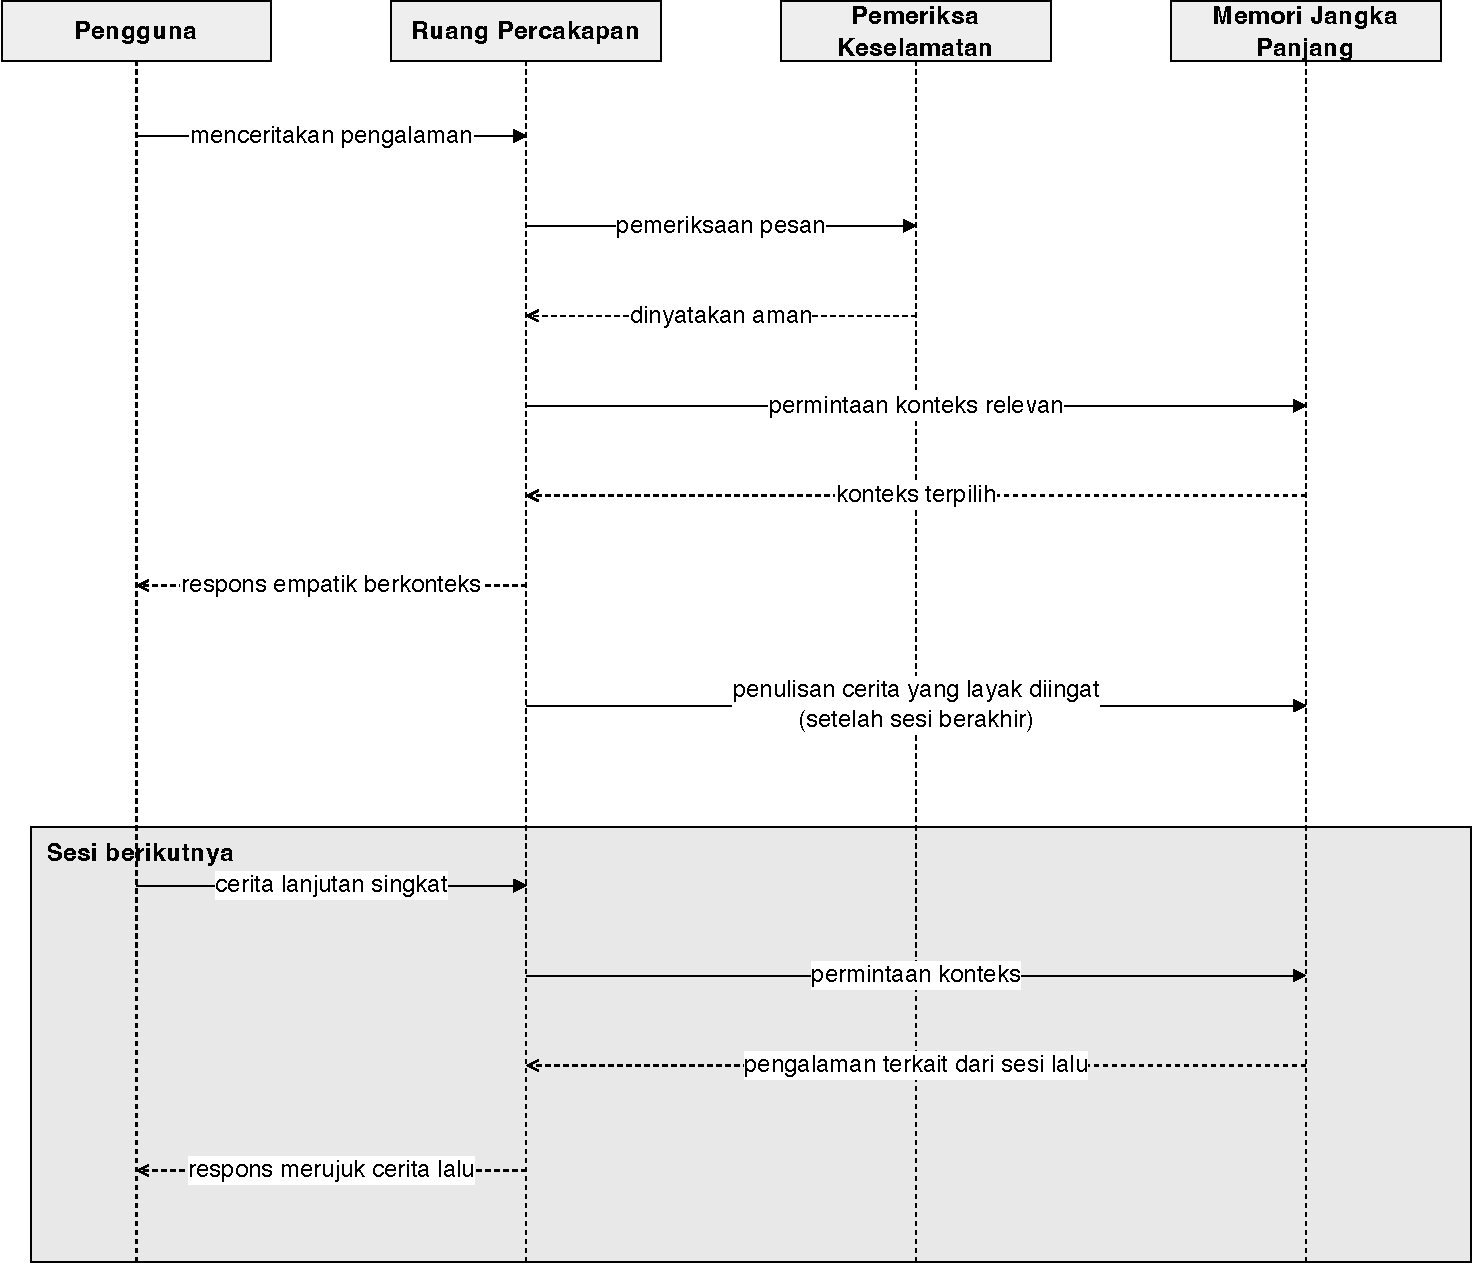
\includegraphics[width=0.95\textwidth]{figures/seq_memory_concept.pdf}
  \caption[Diagram sequence kesinambungan memori]{Diagram \textit{sequence} konseptual kesinambungan memori AXIS pada dua sesi percakapan.}
  \label{fig:seq-memory-concept}
\end{figure}

\subsection{Batas Percakapan dan \textit{Guardrail}}
\label{sec:rancangan-guardrail}
\label{subsec:rancangan-empat-lapis}
\label{subsec:rancangan-tier-crisis}

Rancangan berikut menjawab K4 pada Tabel~\ref{tab:kebutuhan-solusi}. \textit{Guardrail} pada AXIS ditempatkan sebagai batas percakapan yang menjaga peran non-klinis. Batas ini bukan kontribusi utama yang berdiri sendiri, tetapi bagian yang harus ada karena sistem berinteraksi dengan cerita emosional. Mengikuti prinsip \textit{defense in depth} pada Subbab~\ref{sec:guardrail}, rancangan ini dibuat empat lapis: lapisan pertama berupa batasan ruang lingkup yang ditanamkan pada instruksi dasar sistem, lapisan kedua berupa pemeriksaan kata kunci sensitif pada pesan masuk, lapisan ketiga berupa pengenalan sinyal krisis yang disampaikan secara halus atau tidak langsung, dan lapisan keempat berupa peninjauan luaran model bahasa secara independen sebelum sampai ke pengguna. Alur pemeriksaannya ditunjukkan pada Gambar \ref{fig:guardrail-concept-flow}.

\begin{figure}[!htbp]
  \centering
  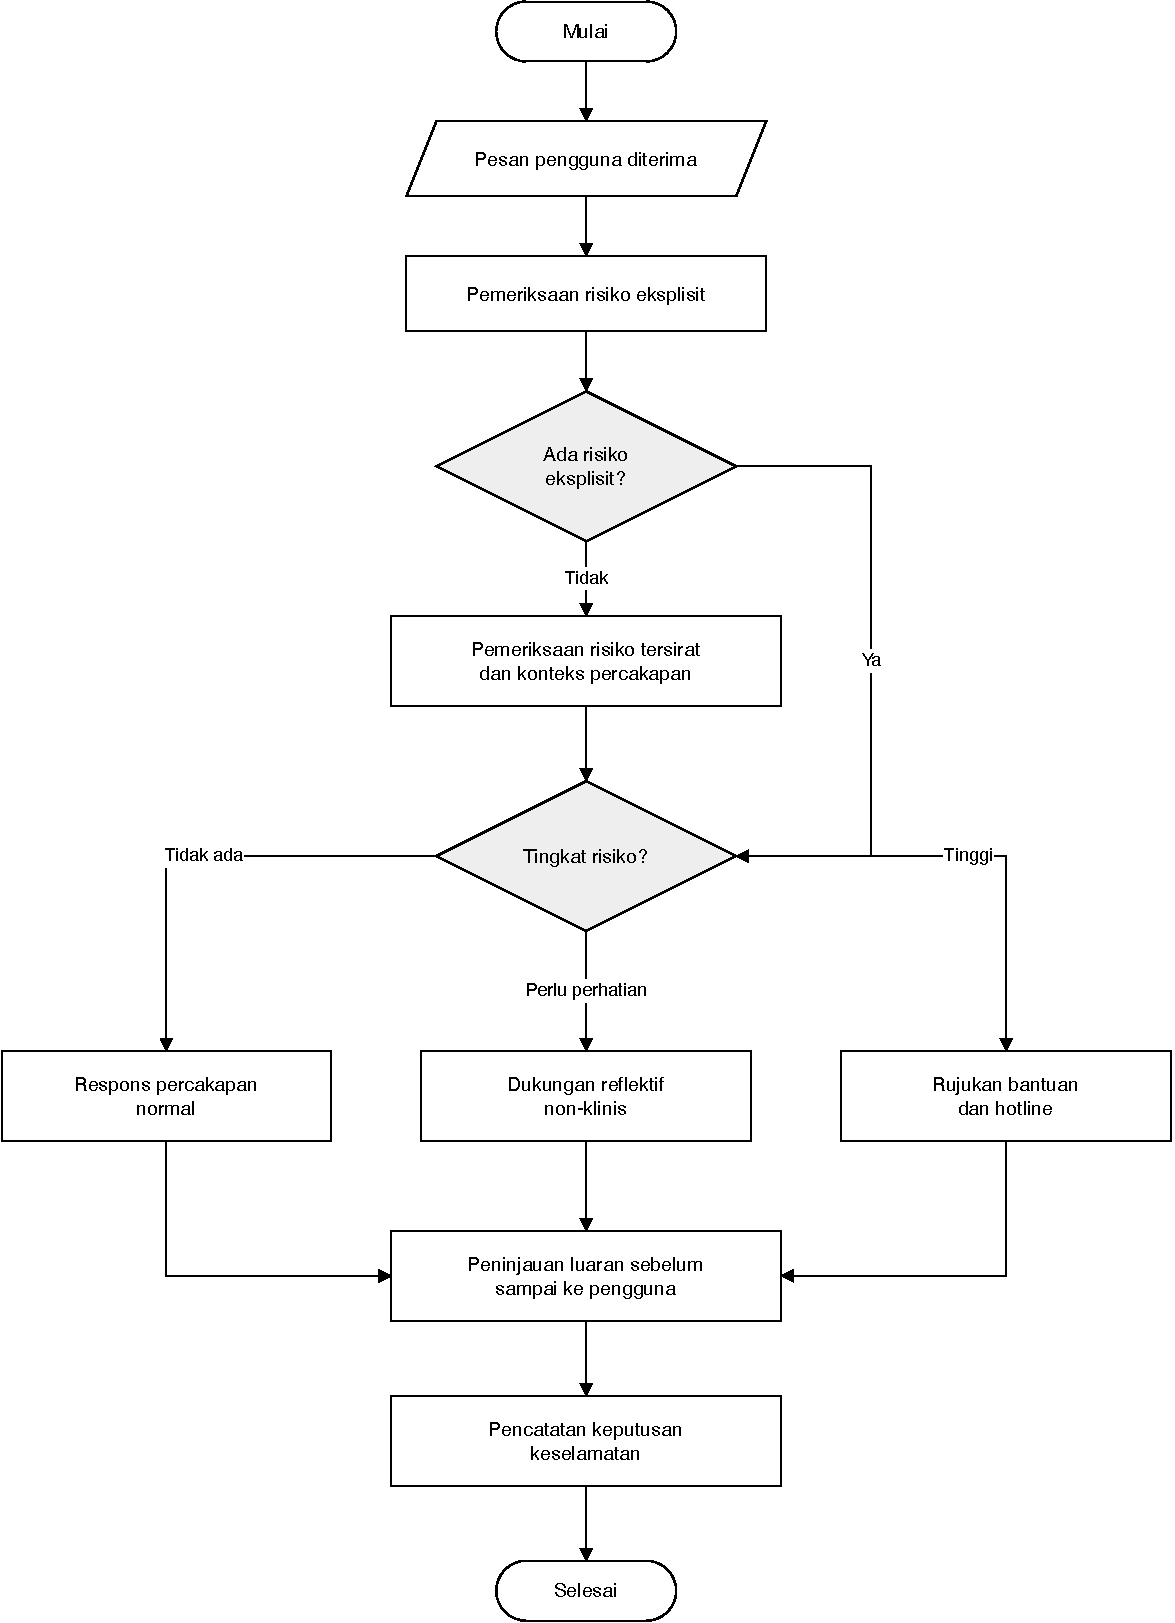
\includegraphics[width=0.85\textwidth]{figures/guardrail_concept_flow.pdf}
  \caption[Flowchart konseptual \textit{guardrail} AXIS]{\textit{Flowchart} konseptual \textit{guardrail} AXIS dari pesan pengguna hingga respons normal, dukungan aman, atau rujukan bantuan.}
  \label{fig:guardrail-concept-flow}
\end{figure}

Pada percakapan biasa, \textit{guardrail} tidak boleh membuat AXIS terasa seperti sistem pengawasan. Pada distres umum, AXIS tetap memberi respons empatik tanpa membuat klaim klinis. Pada risiko tinggi, respons perlu menjadi lebih langsung, lebih aman, dan mengarahkan pengguna ke bantuan profesional. Dengan cara ini, keselamatan tidak menghapus peran \textit{companionship}, tetapi menentukan batas agar pendampingan tetap bertanggung jawab.

\section{Rancangan Evaluasi}
\label{sec:rancangan-evaluasi}

Evaluasi dirancang sebagai arsitektur bukti yang langsung mengikuti klaim pada tiga rumusan masalah. Bukti primer berasal dari pengujian kontrak, \textit{benchmark} berlabel, penilaian buta, dan ablasi terkendali. Studi kasus naratif hanya digunakan sebagai ilustrasi perilaku sistem, sedangkan pengujian pengguna nyata digunakan untuk menilai pengalaman awal memakai purwarupa.

Lima blok evaluasi digunakan sebagai berikut.

\begin{enumerate}[label=\arabic*.,leftmargin=*,itemsep=4pt]
  \item \textbf{Validasi kontrak sistem.} Pengujian unit dan integrasi memeriksa transisi, rute, persistensi, dan operasi data yang memiliki keluaran benar atau salah secara eksplisit. Blok ini membuktikan kesesuaian implementasi terhadap rancangan, bukan kualitas respons terbuka.

  \item \textbf{\textit{Benchmark} berlabel.} Korpus yang dibekukan digunakan untuk menguji deteksi risiko, pemetaan jawaban bebas PHQ-9, penulisan graf memori, \textit{retrieval}, pembaruan \textit{lifecycle}, dan penggunaan memori pada jawaban. Untuk kontrak yang memiliki keluaran deterministik, label acuan ditetapkan langsung dari aturan instrumen dan skenario. Untuk keluaran terbuka, label referensi operasional disusun dengan pedoman tertulis, dua konfigurasi model penilai yang berbeda, dan penentuan akhir oleh model ketiga pada kasus yang tidak selaras.

  \item \textbf{Penilaian buta respons.} Respons AXIS dan \textit{baseline} untuk skenario yang sama diacak serta disembunyikan identitasnya. Dua konfigurasi \textit{LLM-as-judge} menerapkan rubrik ordinal untuk validasi emosi, pemahaman konteks, eksplorasi, ketepatan CBT, batas non-klinis, kesesuaian ragam bahasa, dan \textit{groundedness} ketika memori digunakan. Ketidaksesuaian yang material diperiksa oleh konfigurasi penilai ketiga.

  \item \textbf{Ablasi terkendali.} Kondisi retrieval vektor saja dibandingkan dengan retrieval hibrid menggunakan korpus, kueri, model, prompt, parameter decoding, jumlah kandidat, dan batas konteks yang sama. Perbandingan dilakukan berpasangan pada tingkat kueri.

  \item \textbf{Pengujian pengguna nyata.} Mahasiswa menggunakan purwarupa untuk menilai kegunaan, rasa didampingi, kejelasan skrining, kesinambungan memori, dan pemahaman kendali data. Hasilnya dibaca sebagai pengalaman awal penggunaan, bukan bukti efektivitas klinis.
\end{enumerate}

Korpus, \textit{prompt}, profil model, konfigurasi decoding, dan versi artefak dibekukan sebelum evaluasi. Hasil kuantitatif dilaporkan bersama interval kepercayaan ketika relevan. Penilaian otomatis melaporkan kesepakatan antarkonfigurasi model penilai; pengujian pengguna nyata tetap mengumpulkan persepsi mahasiswa melalui kuesioner. Hasil yang berkaitan dengan domain bahasa dilaporkan menurut ragam formal, informal, bahasa campur, dan eufemistik.

Hubungan antara klaim, unit evaluasi, dan bukti utama dirangkum pada Tabel~\ref{tab:pemetaan-rumusan-rancangan}.

\begin{table}[!htbp]
\centering
\caption{Pemetaan klaim penelitian dan rancangan evaluasi}
\label{tab:pemetaan-rumusan-rancangan}
{\footnotesize
\begin{tabularx}{\textwidth}{|>{\raggedright\arraybackslash}p{2.3cm}|>{\raggedright\arraybackslash}p{3.2cm}|>{\raggedright\arraybackslash}X|}
\hline
\rowcolor{tableheadgray}
\textbf{Klaim} & \textbf{Unit evaluasi} & \textbf{Bukti dan metrik utama} \\
\hline
RM1a: kualitas respons suportif & Respons AXIS dan \textit{baseline} pada skenario yang sama & Penilaian buta dengan rubrik ordinal berbasis EPITOME dan dimensi tambahan; median atau distribusi per dimensi; preferensi berpasangan; \textit{weighted kappa} atau Krippendorff's alpha \\
\hline
RM1b: keselamatan percakapan & Pesan berisiko tinggi dan pesan pembanding tanpa risiko & Sensitivitas sebagai metrik primer; spesifisitas; presisi; $F_2$; jumlah \textit{false negative}; kepatuhan respons aman \\
\hline
RM1c: kesesuaian ragam bahasa & Skenario formal, informal, bahasa campur, dan eufemistik & Skor kesesuaian bahasa dan preferensi per ragam; metrik keselamatan dilaporkan per ragam \\
\hline
RM2: penyampaian skrining PHQ-9 & Transisi orkestrasi, jawaban bebas, skor total, dan item kesembilan & Tingkat kelulusan kontrak; \textit{quadratic weighted kappa}; \textit{macro-F1}; akurasi; ICC dan Bland--Altman bila tersedia data berpasangan; sensitivitas, spesifisitas, dan ketepatan rute item kesembilan \\
\hline
RM3: memori jangka panjang & Penulisan, retrieval, pembaruan, penggunaan, dan ablasi & Presisi, \textit{recall}, dan \textit{macro-F1} node serta relasi; \textit{P@5}, \textit{Recall@5}, MRR, nDCG@5; \textit{update correctness}; \textit{stale-memory rate}; \textit{grounded-answer rate}; kontradiksi; \textit{false-personalization rate}; selisih berpasangan dan 95\% CI \\
\hline
K5: kendali pengguna sebagai kebutuhan pendukung & Tugas pengelolaan memori dan data personal & Kelulusan kontrak fungsional, keberhasilan tugas pengguna, dan pemahaman kontrol; tidak diperlakukan sebagai rumusan masalah terpisah \\
\hline
\end{tabularx}
}
\end{table}
